%!TEX root = da-screen.tex

\chapter{Introduction and Preliminaries}

\section{Scope}

This course focuses on the \emph{theoretical foundations of distributed systems}. Our approach is similar to typical courses on models of computation, computational complexity, and design and analysis of algorithms. The main difference is in the models of computation that we study: instead of traditional models, such as finite state machines, Turing machines, RAM machines, or Boolean circuits, our model of choice is a \emph{distributed system}.

\subsection{Distributed Systems as a Model of Computation}\label{ssec:prelim-model}

A distributed system consists of multiple machines that are connected to each other through communication links. We usually view a distributed system as a (simple, undirected) graph $G = (V,E)$: each node $v \in V$ represents a machine and an edge $\{u,v\} \in E$ represents a communication link between machines $u$ and~$v$.

To understand the key difference between distributed systems and more familiar models of computation, let us consider an illustrative example: the problem of finding a maximal independent set.

An \emph{independent set} for a graph $G = (V,E)$ is a set $I \subseteq V$ such that for each edge $\{u,v\} \in E$ at most one of $u$ and $v$ is in $I$. An independent set $I$ is \emph{maximal} if it cannot be extended, i.e., it is not a proper subset of another independent set.
\begin{center}
    \includegraphics[page=\PIndependentSet]{figs.pdf}
\end{center}

Now given any model of computation $X$ we can pose the familiar question:
\begin{itemize}
    \item \emph{Computability:} is it \emph{possible} to find a maximal independent set in model $X$?
    \item \emph{Computational complexity:} can we find a maximal independent set \emph{efficiently} in model $X$?
\end{itemize}
We are familiar with such questions in the context of Turing machines, but it is not immediately obvious what these questions mean in the context of distributed systems. The following informal comparison illustrates the key differences.
\begin{description}
    \item[Input.] The input is a graph~$G$.
    \begin{descriptionb}
        \item[Turing machines:] We assume that the structure of $G$ is encoded as a string and given to the Turing machine on the input tape.
        \item[Distributed systems:] We assume that the structure of the input graph $G$ is the same as the structure of the distributed system. Initially, each machine $v \in V$ only knows some local information related to $v$ (for example, the degree of $v$ and the unique identifier of $v$). To acquire more information about $G$, the nodes need to exchange messages.
    \end{descriptionb}
    \item[Output.] The output is an independent set $I \subseteq V$.
    \begin{descriptionb}
        \item[Turing machines:] We require that the machine prints an encoding of $I$ on the output tape.
        \item[Distributed systems:] We require that each node $v \in V$ produces one bit of output: if $v \in I$, node $v$ has to output $1$, and if $v \notin I$, node $v$ has to output $0$.
    \end{descriptionb}
    \item[Algorithm.] We say that an algorithm solves the problem if it produces a valid output for any valid input.
    \begin{descriptionb}
        \item[Turing machines:] The algorithm designer chooses the state transitions of the Turing machine.
        \item[Distributed systems:] The algorithm designer writes one program. The same program is installed in each $v \in V$.
    \end{descriptionb}
    \item[Complexity measures.] There are many possible complexity measures, but perhaps the most commonly used is the time complexity.
    \begin{descriptionb}
        \item[Turing machines:] Time = number of elementary steps. In each time unit, (1)~the machine moves the tape heads, (2)~performs a state transition that depends on the contents of the tapes, and (3)~possibly halts.
        \item[Distributed systems:] Time = number of synchronous communication rounds. In each time unit, all machines in parallel (1)~exchange messages with their neighbours, (2)~perform state transitions that depend on the messages that they received, and (3)~possibly halt.
    \end{descriptionb}
\end{description}
To oversimplify a bit, distributed computation is not really about \emph{computation}\mydash it is all about \emph{communication}. Throughout this course, we will see striking examples of the implications of this change of perspective.


\subsection{Outside the Scope}

The term ``distributed computing'' is overloaded, and it means very different things to different people.

For the general public, distributed computing often refers to large-scale high-performance computing in a computer network; this includes scientific computing on grids and clusters, and volunteer computing projects such as SETI@Home and Folding@Home. However, this is \emph{not} the definition that we use, and our course is in no way related to large-scale number crunching.

In general, our focus is on theory, not practice. For our purposes, a communication network is an idealised abstraction. We are not interested in any implementation details or engineering aspects. For example, the following topics are \emph{not} covered on this course: physical properties of wired or wireless media, modulation techniques, communication protocols, standards, software architectures, programming languages, software libraries, privacy, and security.

Within the field of the theory of distributed computing, there are also numerous topics that we are not going to cover. We will conclude this course with a brief overview of other research areas within the field in Section~\ref{sec:other-stuff}.


\chapter{What Next?}

\section{Other Stuff Exists}\label{sec:other-stuff}

Distributed computing is a vast topic. We conclude this course by mentioning perspectives that we have not covered; we also provide pointers to more in-depth information.

\subsection{Models of Computing}

Many models of distributed computing can be seen as extensions of the models that we have studied. The following extensions are familiar from the context of classical computational complexity and Turing machines.
\begin{description}
    \item[Randomised algorithms.] Each node has access to a stream of random bits. A good example is Luby's~\cite{luby86simple} randomised algorithm for finding a maximal independent set\mydash the algorithm uses the random bits for symmetry breaking.
    \item[Nondeterministic algorithms.] It is sufficient that there exists a \emph{proof} that can be verified efficiently in a distributed setting; we do not need to construct the proof. This research direction was introduced by Korman et al.~\cite{korman05proof}.
\end{description}

\subsection{Variants}

There are many variants of the model that we described.
\begin{description}
    \item[Asynchronous systems.] Computers do not necessarily operate in a synchronous manner. In particular, the propagation delays of the messages may vary.
    \item[Message passing vs.\ shared memory.] Our model of computing can be seen as a \emph{message-passing system}: nodes send messages (data packets) to each other. A commonly studied alternative is a system with \emph{shared memory}: each node has a shared register, and the nodes can communicate with each other by reading and writing the shared registers.
\end{description}
The above aspects were irrelevant for our purposes, as we were only interested in the number of communication rounds; for example, asynchronous systems can be ``synchronised'' efficiently~\cite{awerbuch85complexity}. However, if we consider other complexity measures or fault tolerance, such details become important.

Our model of computing is primarily intended to capture the specifics of \emph{wired} networks\mydash communication links can be seen as cables that connect the computers. There are also numerous models that are designed with \emph{wireless} networks in mind. A simple graph is no longer an appropriate model: a single radio transmission can be received by multiple nodes, and multiple simultaneous radio transmissions can interfere with each other. Radio propagation is closely connected with physical distances; hence in the context of wireless networks one often makes assumptions about \emph{physical locations} of the nodes.

\subsection{Complexity Measures}\label{ssec:next-compl-meas}

For us, the main complexity measure has been the number of synchronous communication rounds. Naturally, other possibilities exist.
\begin{description}
    \item[Space.] How many bits of memory do we need per node?
    \item[Number of messages.] How many messages do we need to send in total?
    \item[Message size.] We did not limit the size of a message. However, it is common to assume that the size of each message is $O(\log n)$ bits; how many communication rounds do we need in that case?
\end{description}

\subsection{Fault Tolerance and Dynamics}\label{ssec:next-fault}

Fault tolerance in general is an important topic in any large-scale distributed system. In the theory of distributed computing, fault tolerance has been studied from many different and complementary perspectives, of which we mention three representative examples.
\begin{description}
    \item[Dynamic networks.] Nodes can join and leave; edges can be removed and added. The system is expected to correct the output quickly after each change.
    \item[Byzantine failures.] A fraction of nodes can be malicious and they may try to actively disturb the algorithm. Nevertheless, non-malicious nodes must be able to produce a correct output.
    \item[Self-stabilising systems.] The initial state of each node can be arbitrary\mydash an adversary may have corrupted the memory of each node. Nevertheless, the system must eventually recover and produce a correct output. Note that a self-stabilising system can never stop; all nodes have to keep communicating with each other indefinitely. See Dolev's~\cite{dolev00self-stabilization} textbook for more information.
\end{description}

\subsection{Problems}

In this course we have studied \emph{input/output problems}: we are given an input, we expect the system to do some computation, and eventually the system has to produce a correct output.

We assumed that the input is equal to the structure of the communication graph. This is not the only possibility: in general, one can solve arbitrary input/output problems in a distributed manner.

However, there are also many problems that are \emph{not} input/output problems. In the context of distributed algorithms, there are also problems that are related to \emph{controlling} an autonomous entity. Often we will use the metaphor of robot navigation: the graph is a map of an environment, and we need to control ``robots'' that navigate in the graph\mydash however, instead of a physical robot, we can equally well study a logical entity such as a data packet or a token that is routed throughout a network. Some examples of robot navigation tasks include the following.
\begin{description}
    \item[Graph exploration.] A robot needs to visit all nodes of a graph.
    \item[Rendezvous.] There are two robots who need to meet each other at a single node.
\end{description}

